\documentclass[conference]{IEEEtran}

\usepackage{listings}
\usepackage{pgfplots}
\usepackage{hyperref}
\usepackage{caption}
\usepackage{subcaption}

\usepackage[
  backend=biber,
  style=ieee,
  sorting=none
]{biblatex}
\addbibresource{CAD.bib}

\usepackage{c/style} % include custom style for C.
\lstset{basicstyle=\footnotesize\ttfamily,
  breaklines=true}




\begin{document}

\title{Performance enhancement using CUDA in a simulation of heat diffusion}

\author{
\IEEEauthorblockN{Gonçalo Lourenço \\ nº55780 \\ gm.lourenco@campus.fct.unl.pt}
\and
\IEEEauthorblockN{Joana Faria \\ nº55754 \\ js.faria@campus.fct.unl.pt}
}

\maketitle



\section{Introduction}
This assignment aims to optimize a base code, written in \texttt{C}, that computes a simulation for heat diffusion. For the optimization, we seek to take advantage of GPU programming using \texttt{CUDA}, and explore several alternatives to find the most efficient one.

To find the best performance we will explore different approaches, namely analyzing different configurations, exploring the impact of using shared memory, and the difference between using streams and not.

Knowing that the architecture of the system influences the performance obtained, the first step of our work is to understand the architecture of the system where our program will run. So we present the characteristics below:
\lstinputlisting{infoDevice}

\section{Results}
To accurately compare the different versions all the tests were performed in the university cluster and averaged the execution times over ten execution. The parameters chosen were:
\lstinputlisting[language=C,style=c, firstline=71, lastline=76]{../proj1/main.c}


\subsection{Sequential Verion}
We start by analyzing and profiling the sequential version to understand what improvements can be done, and what parts are the more problematic.

By a quick analysis of the code, we expect the cycle present in the \texttt{main} function to be the biggest problem. This assumption is supported by the reports of the profiling tools. The output of these tools can be seen in the files \texttt{results/sequential/gprof} and \texttt{results/sequential/perf}.

The average execution time obtained with this version is 153.979 seconds.

\subsection{V1 Version}
Next, we make a naive translation of the sequential code to \texttt{CUDA} code, which can be found in \texttt{proj1/v1.cu}. This implementation was based on the tutorial provided with the project, with some adaptations.\cite{SolvingHeatEquation}

With this version, we experimented with a variety of grid configurations. We follow \texttt{Nvidia} recommendations\cite{CUDABestPractices}:

\begin{itemize}
  \item Threads per block should be a multiple of warp size to avoid wasting computation on under-populated warps and to facilitate coalescing.
  \item A minimum of 64 threads per block should be used, and only if there are multiple concurrent blocks per multiprocessor.
  \item Between 128 and 256 threads per block is a good initial range for experimentation with different block sizes.
\end{itemize}

So we start with a configuration having 256 threads per block and we test until the maximum of 1024 threads per block. We didn't find significant differences between these configurations.

For the sake of completeness, we tested with blocks smaller than 68 threads, and, as expected, we got worse results. The results are summarized in \autoref{fig:executionTimeV1}


\begin{figure}[ht]
  \centering
  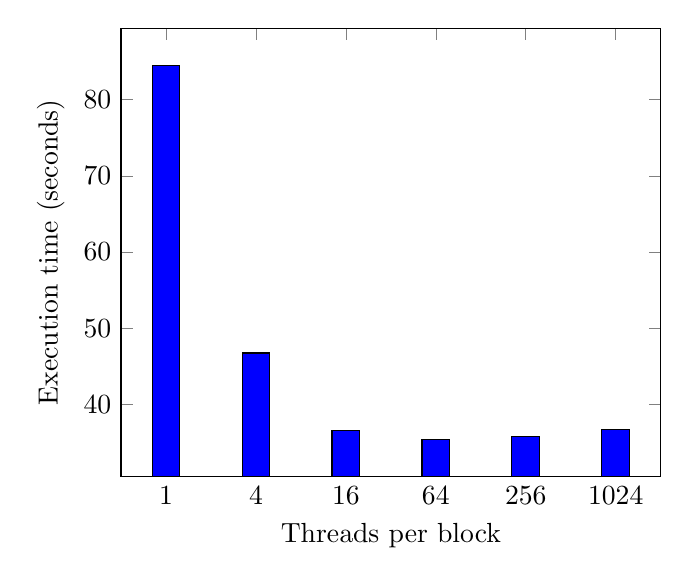
\begin{tikzpicture}

    \begin{axis}[
        ylabel={Execution time (seconds)},
        xlabel={Threads per block},
        symbolic x coords={1,4, 16, 64, 256, 1024},
        xtick=data
      ]
      \addplot[ybar,fill=blue] coordinates {
          (1,   84.463241)
          (4,   46.764692)
          (16,  36.538622)
          (64,   35.454548)
          (256,   35.763267)
          (1024,   36.727775)
        };
    \end{axis}
  \end{tikzpicture}
  \caption{Execution time of different grid configurations for V1}
  \label{fig:executionTimeV1}
\end{figure}

Analyzing this version using the profiling tool \texttt{NVPROF} we can conclude that the majority of execution time is spent in communication between the host and the device, with only  22.19\% of the execution time dedicated to kernel execution. The program spends 41.74\% of time copying data from the host to the device and 36.07\% from the device to the host. The complete results are available at \texttt{results/v1/nvprof\_results}.

\subsection{V2 Version}
In this version, we intend to improve the previous naive implementation, reducing the communication between the host and the device, which we detect to be a big problem in the previous version. In this problem, there aren't any computations needed between the steps so we don't need to transfer the data to the host between steps.

As expected we got a huge improvement in execution time. This version has an average execution time of 2.106914 seconds. Using \texttt{NVPROF} we can see that now the kernel is executing 100.00\% of the total execution time. The full report is in \texttt{results/v2/nvprof\_results}.

we decided from now on to increase the complexity of the problem by increasing the amount of work. So the new parameters are:

\lstinputlisting[language=C,style=c, firstline=100, lastline=105]{../proj1/v2.cu}


\section{Results}

\begin{figure}[ht]
  \centering
  \begin{subfigure}[b]{0.24\textwidth}
    \resizebox{\textwidth}{!}{%
    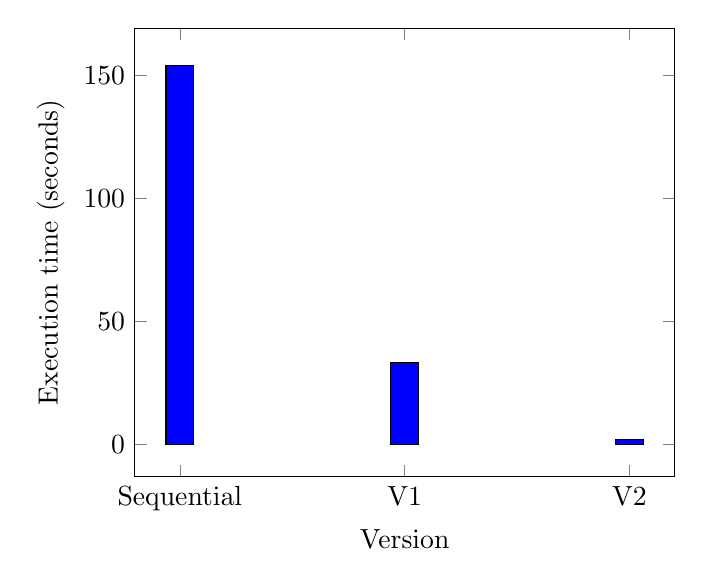
\begin{tikzpicture}

      \begin{axis}[
          ylabel={Execution time (seconds)},
          xlabel={Version},
          symbolic x coords={Sequential, V1, V2},
          xtick=data,
        ]
        \addplot[ybar,fill=blue] coordinates {
            (Sequential,   153.979491)
            (V1,  33.376915)
            (V2,   2.106914)
          };
      \end{axis}
    \end{tikzpicture}
    }%
    \caption{Execution time of sequential version, V1 e V2}
    \label{fig:executionTimeCompareA}
  \end{subfigure}
  \begin{subfigure}[b]{0.24\textwidth}
    \resizebox{\textwidth}{!}{%
    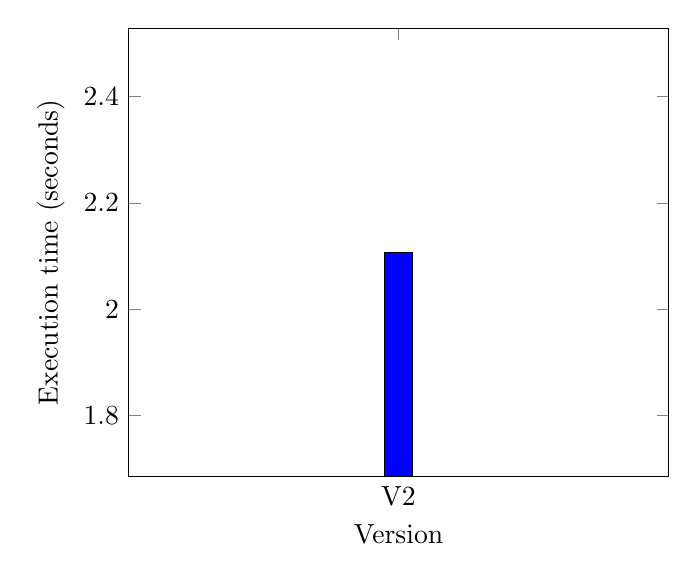
\begin{tikzpicture}

      \begin{axis}[
          ylabel={Execution time (seconds)},
          xlabel={Version},
          symbolic x coords={V2},
          xtick=data
        ]
        \addplot[ybar,fill=blue] coordinates {
            (V2,   2.106914)
          };
      \end{axis}
    \end{tikzpicture}
    }%
    \caption{Execution time of V2, V3, V4 and V5}
    \label{fig:executionTimeCompareB}
  \end{subfigure}
  
  \caption{Execution time of the different versions}
  \label{fig:executionTimeCompare}
\end{figure}






\printbibliography


\end{document}